\documentclass{article}
    % General document formatting
    \usepackage[margin=0.5in]{geometry}
    \usepackage[parfill]{parskip}
    \usepackage[utf8]{inputenc}
    \usepackage[T2A]{fontenc}
    \usepackage[english,russian]{babel}
    
    % Related to math
    \usepackage{amsmath,amssymb,amsfonts,amsthm}

    \usepackage{tikz}
    \usetikzlibrary{patterns}
    \usepackage{graphicx}

    \usepackage{subfigure}
    \usepackage{graphicx}
    \graphicspath{{media/}}

    % \newcommand{\argmin}{\mathop{\mathrm{arg\,min}}
    \DeclareMathOperator*{\argmin}{arg\,min}

\begin{document}

\section{Введение}

\section{Постановка задачи}

Пусть на эвклидовой плоскости
$\mathbb R$ задано $n$ плоских деталей
$A_1, A_2, \dots A_n$,
ограниченных $k$ замкнутыми попарно не пересекающимися контурами
$C_1, C_2, \dots C_k$,
таким образом
$$
\bigcup_{i=1}^n \delta A_i = \bigcup_{j=1}^k C_k
$$
Сами замкнутые контуры состоят из конечного числа
отрезков прямых линий и дуг окружностей.

Для упрощения задачи мы будем считать,
что резка ведётся не по эквидистантному контуру,
а непосредственно по контуру детали:
сегмент резки
$S_i = C_i, \forall i=\overline{1, k}$
и точка врезки $M_i$ всегда совпадает с точкой выключения
инструмента и тоже лежит непосредственно
на контуре:
$M_i \equiv M_i^* \in C_i, \forall i = \overline{1, k}$.

Также будем считать заданной точку начала маршрута резки $M_0$.

В этих обозначениях задача CCP
(Continous Cutting Problem)
заключается в нахождении
\begin{enumerate}
    \item{$k$ точек врезки $M_i \in C_i$}
    \item{Порядка обхода контуров $C_i$,
    то есть перестановки $k$ элементов
    $I=(i_1, i_2, \dots, i_k),
    i_j \in \overline{1,k}, \forall j \in \overline{1,k}$}
\end{enumerate}

В качестве целевой функции берём время резки,
в общем виде:
$$
T = \frac{1}{V_{on}} \sum_{j=1}^k |C_{i_j}| +
\frac{1}{V_{off}} \sum_{j=0}^k |\overrightarrow{M_{i_j} M_{i_{{j+1}}}}|
$$
где $V_{on}$ и $V_{off}$ --
скорость резки и холостого хода соответственно. 
Также будем считать для краткости,
что
$M_{i_0} = M_{i_{k+1}} = M_0$.

В данном случае можно упростить целевую функцию
до длины холостого хода:
$$
\mathcal L = \sum_{j=0}^k |\overrightarrow{M_{i_j} M_{i_{{j+1}}}}|
$$
$$
\mathcal L \to \min
$$

При решении данной задачи мы будем дополнительно
соблюдать
\textit{ограничение предшествования},
которое традиционно формулируется в виде двух правил:
\begin{enumerate}
\item{}
Если деталь ограничена внешним контуром и одним
или несколькими внутренними контурами
(содержит отверстия),
то внутренние контуры должны
быть вырезаны до того,
как будет завершена резка внешнего контура
\item{}
Если деталь расположена в отверстии
другой детали
(внутри её внутреннего контура),
то внутренняя деталь
должна быть вырезана до того,
как будет завершена резка
содержащего её контура
(другой детали)
\end{enumerate}

В данном случае эти условия упрощаются до одного:
если некоторый контур расположен внутри другого,
то он должен быть вырезан раньше его:
$$
\tilde C_a \subset \tilde C_b
\Rightarrow
i_a < i_b
$$
где под
$\tilde C_i$ понимается фигура,
ограниченная контуром $C_i$.

В такой формулировке ограничение предшествования
ограничивает множество возможных перестановок
$I=(i_1, i_2, \dots, i_k)$,
входящих в полное решение задачи
$\big<
i_1, i_2, \dots i_k,
M_1, M_2, \dots M_k
\big>$.

Традиционным способом решения сформулированной задачи CCP
является сведение её к обобщённой задаче коммивояжера
(Generalized Traveling Salesman Problem, GTSP)
путём дискретизации контуров
$C_i, i=\overline{1, k}$
с некоторым шагом $\varepsilon$
и последующим выбором точек врезки
$M_i$ из конечного множества кандидатов.

В данной статье мы вместо этого решаем задачу непрерывной оптимизации
для поиска точек врезки $M_i$.

\section{Непрерывная оптимизация}
В практических приложениях
форма контуров деталей ограничена
набором отрезков прямых линий и дуг окружностей.
В этих условиях оказывается возможным
точно решить задачу нахождения
\textit{одной} точки врезки
при фиксированном положении всех остальных $M_i$,
а также порядка обхода $I=(i_1, i_2, \dots, i_k)$.
$$
\mathcal L \to \min_{M_i}
$$
что упрощается до
$$
\sqrt{\overrightarrow{M_i M_{i-1}}^2} +
\sqrt{\overrightarrow{M_i M_{i+1}}^2} \to
\min_{M_i \in C_i}
$$
Простейший геометрический анализ показывает,
что если соседние
(считающиеся известными)
точки врезки расположены
\textit{с одной стороны}
сегмента контура
(точнее, содержащей его линии или окружности),
то точное решение оптимизационной задачи
находится как пересечение
соединяющей линии $M_{i-1}M_{i+1}$
с прямой или окружностью,
на которой лежит сегмент.

Если же обе точки находятся
\textit{с одной стороны},
то решение находится при помощи принципа Ферма,
так чтобы соблюдалось правило
\textit{угол падения равен углу отражения},
как это можно видеть на рис. \ref{fermat}.

По аналогии с ALS
(Alternating Least Squares)
оказывается возможным использовать
процесс,
который можно было бы назвать
\textit{Alternative Fermat Principle}:
\begin{itemize}
    \item{}
    Начальные положения точек врезки 
    $M_i \in C_i$
    выбираются
    (для каждого контура)
    случайным образом
    \item{}
    $\forall i \in \overline{1,k}$
    решается задача поиска оптимального положения
    \textit{одной} точки врезки $M_i$
    (за константное время $O(1)$)
    \item{}
    Процесс повторяется до схождения
    по позициям всех точек врезки
    (с некоторой наперёд заданной точностью)
\end{itemize}
С практической точки зрения процесс оказывается
очень хорошо сходящимся за время $O(k)$.
Поэтому он используется в качестве одного шага
полного алгоритма непрерывно-дискретной оптимизации.

\begin{figure}
    \begin{center}
    \tikz[rotate=27,scale=1.1]{
        \draw[thick]
            (0, 0) coordinate(zero) -- (5, 0) coordinate(future) node[right] {$S_k$};
        \fill[black] 
            (1.5, 0) circle(0.1) coordinate(middle) node[below right]  {$M_i \equiv M_i^*$}
            (1, 1) circle(0.1) coordinate(from) node[above left] {$M_{i-1}$} ++(-1.5,0) node[above] {$S_{k-1}$}
            (4.5, 2) circle(0.1) coordinate(to) node[above] {$M_{i+1}$} ++(1.5,0) node[below] {$S_{i+1}$};
        \begin{scope}
            \clip (from) circle(1);
            \draw[thick] (from) ++(0, 3) circle(3);
        \end{scope};
        \begin{scope}
            \clip (to) circle(1.5);
            \draw[thick] (to) ++(3, 4) circle(5);
        \end{scope};
        \draw[dashed] (from) -- (middle) -- (to);
        \draw[thin] (4.5, -2) circle(0.062) coordinate(mirror) node[right] {$\hat M_{i+1}$};
        \coordinate (opt) at (intersection of zero--future and mirror--from);
        \draw[thin] (opt) circle(0.1);
        \draw[dotted] 
            (mirror) -- (opt)
            (mirror) -- (to);
        \draw[thin] (from) -- (opt) -- (to);

        \draw[->,>=latex,red,thick] (middle) to[bend right] (opt);
        
    }
    \caption{Принцип Ферма и поиск точки врезки} \label{fermat}
    \end{center}    
\end{figure}

\section{Дискретная оптимизация}

Задача дискретной оптимизации,
решаемая в ходе решения CCP
представляет собой поиск перестановки,
минимизирующей длину холостого хода
$$
\mathcal L \to \min_{i_1, i_2, \dots i_k}
$$
Для её решения применяется метод переменных окрестностей
(VNS, Variable Neighborhood Search)
на множестве перестановок $P_k$.

Общая схема VNS в применении к CCP:
\begin{enumerate}
    \item $ I \gets random P_k$
    \item $ k \gets 1$
    \item \textbf{while} $k < k_{max}$
    \begin{enumerate}
    \item $ I' \gets \argmin\limits_{I' \in \mathcal N^k(I)} \mathcal L(I')$
    \item \textbf{if} $\mathcal L(I') < \mathcal L(I)$
    \begin{itemize}
        \item $I \gets I'$
        \item $ k \gets 1$
    \end{itemize}
    \item \textbf{else}
    \begin{itemize}
        \item $ k \gets k+1$
    \end{itemize}
    \end{enumerate}
    \item \textbf{end}
\end{enumerate}
На шаге (a)
систематически и многократно применяется описанная выше
непрерывная оптимизация,
фактически
$$
\mathcal L(I') = \min_{M_1, M_2, \dots M_k} \mathcal L(M_1, M_2, \dots M_k | I')
$$

Для построения окрестностей
(различной структуры)
применялись разнообразные приёмы
(большая их часть не может быть удобно
получена при помощи популярных метрик):

\begin{itemize}
    \item Все возможные попарные перестановки двух элементов текущей перестановки $I=(i_1, i_2, \dots i_k)$.
    Этот вид окрестности как раз может быть описан при помощи расстояния Левенштейна
    \item Перестановки 3 элементов.
    Практически использовались не все тройные перестановки,
    а ``локальные'',
    у которых расстояние между элементами не превышает
    заданного значения
    (параметра алгоритма)
    \item Аналогично рассматривались перестановки любых
    четырёх элементов,
    находящихся не дальше определённой дистанции
    друг от друга
    \item Циклические перестановки внутри блока произвольной длины
    \item Реверс блока произвольной длины
    \item Перестановки двух блоков одинаковой длины
    \item Циклический сдвиг цепочки блоков одинаковой длины
    \item Порядка десяти других вариантов построения окрестности перестановки $\mathcal N(I)$
\end{itemize}

В случае,
если какой-то из рецептов генерирует
окрестность слишком большого 
(с практической точки зрения)
размера,
последняя всегда может быть
ограничена при помощи какой-нибудь простой эвристики,
подобно тому,
как это описано для 
тройных и четверных перестановок.

Кроме того,
могут применяться разнообразные варианты
техники переменных окрестностей,
такие как
First Improvement
(вместо описанного выше Best Improvement)
либо стохастические методы выбора
точки в текущей окрестности.
Влияние этих методов
на производительность алгоритма
должно стать предметом дальнейших исследований.

\section{Учёт ограничений предшествования}

Описанные до сих пор шаги алгоритма 
можно считать одним из способов решения
задачи коммивояжера
(TSP, Traveling Salesman Problem)
с не вполне эвклидовым расстоянием
между городами.

Особенностью же задач оптимизации
маршрута резки является то,
что они содержат целый ряд дополнительных
ограничений на допустимые решения,
вызванные технологическими особенностями
процесса резки листовых материалов.

Одним из наиболее известных таких
ограничений является формализованное выше
ограничение предшествования.

В предложенном алгоритме оно может быть
легко учтено.

Для этого предварительно из всех контуров отбросим
те, внутри которых содержатся другие контура и построим
новое множество:
$$
\big\{
    C_i | \forall j \ne i: C_j \cap \tilde C_i = \varnothing
\big\}
$$
Для этого множества контуров решим задачу 
непрерывно-дискретной оптимизации,
как описано выше.

Легко заметить, 
что полученный путь
\begin{equation}
    \bigcup_{i=0}^{k'} M_i M_{i+1} 
\label{path-found}
\end{equation}
пересекается со \textbf{всеми}
исходными контурами $C_i, i \in \overline{1,k}$ --
с отобранными на первом шаге по построению,
а с остальными
(внешними по отношению к отобраным),
потому что исходная и конечная точка
$M_0 \equiv M_{k+1}$
находится снаружи всех контуров,
а внутри каждого из внешних контуров
есть хотя бы один контур,
через который проходит маршрут
(\ref{path-found}).

Теперь для каждого контура,
для которого ещё не найдена точка врезки $M_i$
(то есть содержащего другие контуры внутри)
найдём все точки пересечения с маршрутом
(\ref{path-found}),
и поскольку таких точек будет несколько,
выберем из всех самую последнюю
(в смысле направления движения по маршруту).

Маршрут (\ref{path-found}) с добавленными
в него точками врезки и будет полным решением
исходной (полной) задачи,
учитывающим ограничения предшествования.
Его длина очевидно не изменится от вставки
в него дополнительных точек.

Действительно, в нём содержатся все $k$ точек врезки
$M_1, M_2, \dots M_k$
и точки врезки для внешних контуров
по построению достигаются
после точек врезки содержащихся в них внешних контуров.

Кроме того, если решение сокращённой задачи оптимально
(в смысле длины холостого хода),
то и полученное решение полной задачи тоже оптимально.
Действительно,
если бы нашлось более короткое решение полной задачи,
то оставив в нём только точки врезки в отобранные контура
мы получим решение сокращённой задачи,
очевидно имеющее ту же длину,
которая меньше исходной.
А это невозможно ввиду предположения,
что исходное решение оптимально.

Таким образом,
описанный приём позволяет
эффективно учесть ограничения
предшествования в задаче CCP.
Фактически он приводит
к снижению размерности пространства решений,
что может значительно уменьшить время работы алгоритма.

\section{Численные эксперименты}
\begin{figure}
    \begin{center}
    \subfigure[Точное решение GTSP]{
    \resizebox*{0.48\textwidth}{!}{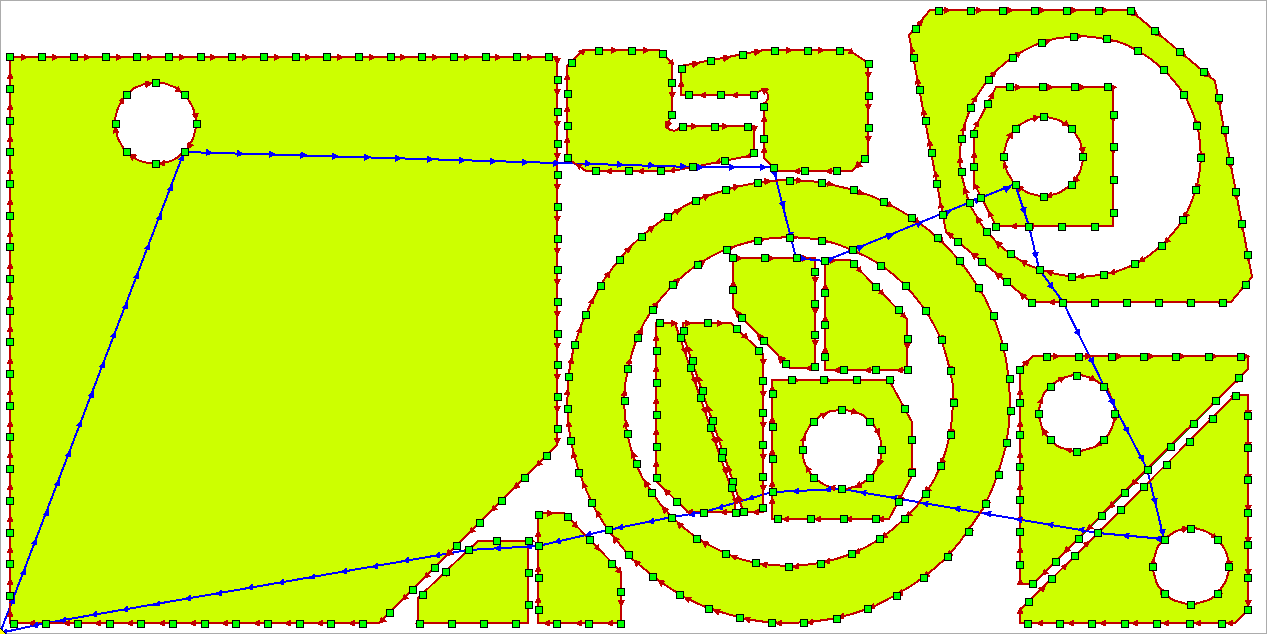
\includegraphics{464-gtsp.png}}}
    \subfigure[Наше решение CCP]{
    \resizebox*{0.48\textwidth}{!}{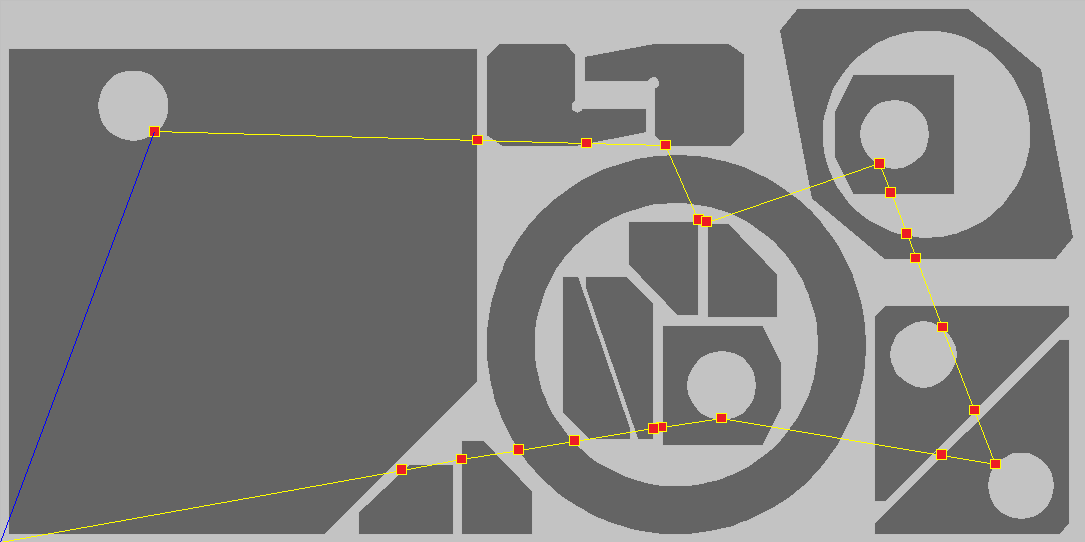
\includegraphics{464-dual.png}}}
    \caption{Задание №464}
    \label{quality}
    \end{center}
\end{figure}

С практической точки зрения предлагаемый алгоритм
оказывается очень удачным
и легко находит хорошие решения,
несмотря на отсутствие математических гарантий этого.

Чтобы подтвердить это,
мы провели ряд экспериментов
для сравнения результатов описанного алгоритма
с другим алгоритмом,
находящим точное решение задачи GTSP
при количестве контуров
(мегаполисов) не более 32.
Результаты в табл. \ref{exact-3}.

\begin{table}[h]
    \begin{center}    
    \begin{tabular}{l|*{3}{r}}
        Задание & №229 & №464 & №3211 \\
        \hline
        Деталей & 11 & 14 & 17\\
        Контуров & 12 & 21 & 22 \\
        $L_{on}$, м & 24.609 & 21.717 & 25.051 \\
        Точек для GTSP & 491 & 429 & 493 \\
        Точное решение GTSP, м & 7.729 & 4.743 & 4.557 \\
        Наше решение CCP, м & 7.727 & 4.706 & 4.536 \\
    \end{tabular}
    \caption{Сравнение с точным решением задачи GTSP}
    \label{exact-3}
    \end{center}
\end{table}

Визуально качество построенного маршрута резки
можно оценить на рис. \ref{quality}.
Видно, что решения практически совпадают.
Длина решения CCP оказывается даже чуть лучше,
чем точное решение GTSP.
Причина в том,
что ввиду дискретизации маршрут,
построенный для GTSP,
вынужден немного отклоняться от прямой линии.

\section{Заключение}

\section{Библиографический список}

\end{document}